\section{Theoretische Grundlagen}
\label{cha:kapitel-2}
Dieses Kapitel soll für ein grundlegendes Verständnis der Architektur von ADF und Grails und des Umfangs dieser Frameworks sorgen, um im nachfolgenden Vergleich (Kapitel \ref{cha:kapitel-3} und \ref{cha:kapitel-4}) der beiden die Vor- und Nachteile nachvollziehen zu können. Hierbei wird zunächst allgemein die Entstehung der Frameworks und die den beiden Frameworks zugrunde liegende MVC-Architektur (Kapitel \ref{sec:entstehung} und \ref{sec:mvc}) erläutert und nachfolgend auf die spezifische Architektur und die jeweiligen Eigenschaften der beiden Frameworks eingegangen (Kapitel \ref{sec:adf} und \ref{sec:grails}).

\subsection{Entstehung}
\label{sec:entstehung}
Mit der Einführung von SOA (Service Oriented Architecture) in der Softwareentwicklung hat die Entwicklung von traditionellen Webanwendungen, in denen die Anwendung eine vollständige Lösung ist, ein Ende gefunden. Moderne Anwendungen sind heute nicht mehr eine vollständige Lösung, sondern sie sind komponentenbasierte Benutzerschnittstellen, die lokale und remote Services für ihre Business Logik verwenden. \autocite[S. XXI]{OFDG2010}
\subsection{MVC Architektur allgemein}
\label{sec:mvc}
Die Model View Controller (MVC) Architektur wurde in den 1970er Jahren von Trygve Reenskaug für die Plattform Smalltalk entwickelt und spielt bis heute eine bedeutende Rolle in den meisten UI-Frameworks und dem UI-Design\autocite[S. 330]{PEAA2002}.
Wie der Name schon vermuten lässt, besteht die MVC Architektur aus drei Rollen, dem Model, dem View und dem Controller.
\begin{itemize}
\item Das Model ist ein nicht sichtbares Objekt, dass einige Informationen der Domäne, wie z.B. alle Daten und Verhalten enthält. Diese Daten und Informationen müssen nicht denen die in der UI verwendet werden entsprechen\autocite[S. 330]{PEAA2002}.

\item Die View dient dazu Informationen aus dem Model anzeigen zu können. Dies kann z.B. in Form einer HTML-Seite geschehen, in der die gewünschten Informationen des Models dann angezeigt werden\autocite[S. 330]{PEAA2002}.

\item Die letzte Rolle ist die des Controllers. Der Controller dient dazu Benutzereingaben anzunehmen, das Model zu manipulieren und das View Objekt zu aktualisieren\autocite[S. 330f]{PEAA2002}.
\end{itemize}
Die wichtigste Trennung ist die Trennung von Model und View. Der Grundgedanke hierbei ist, dass ein Entwickler, wenn er eine View (Ansicht) entwickelt, über andere Dinge nachdenkt, als wenn er das Model entwickelt. Beispielsweise denkt er bei der Entwicklung der View mehr über die Mechanismen der UI und bei der Entwicklung des Models mehr über die Geschäftsstrategie nach. Zudem möchte ein User eventuell ein und dieselbe Information aus dem Model in einer Anwendung auf unterschiedliche Weise dargestellt haben, was sich durch die Trennung von View und Model vereinfacht, da für jede Ansicht das selbe Model verwendet werden kann und sich nur die View ändert. Ein letzter Aspekt, der für die Trennung von Model und View spricht, ist dass nicht sichtbare Objekte meist besser zu testen sind als sichtbare und so durch die MVC-Architektur die Modellogik getrennt von der Benutzeroberfläche (GUI) getestet werden kann.
\begin{figure}[h]
\centering
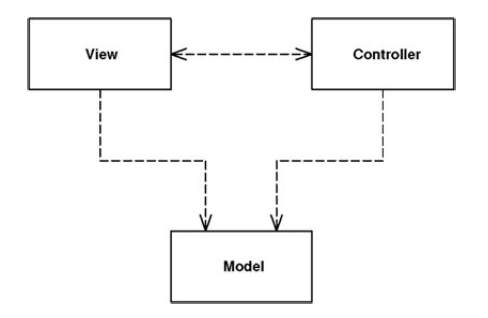
\includegraphics[width=0.80\textwidth]{img/MVC-Allgemein(Fowler).png}
\caption {MVC-Architektur \autocite[S. 330]{PEAA2002}}
\label{fig:mvc}
\end{figure}
Die Trennung von View und Controller dagegen ist weniger relevant und nicht immer sinnvoll, weshalb in einigen Frameworks heute eine Kombination von View und Controller verwendet wird. Selbst in den meisten Versionen von Smalltalk, für die die MVC-Architektur ursprünglich entwickelt wurde, wirde meist eine Kombination von View und Controller verwendet. Die Trennung von View und Controller ist vor allem dann sinnvoll, wenn es sich um Rich-Client-Systeme handelt oder der Controller von Web-Frontends separiert wird. \autocite[S. 330-332]{PEAA2002}\\
Wie auch in der Abbildung \ref{fig:mvc} zu sehen ist, ist die Richtung der Abhängigkeiten für die MVC-Architektur entscheidend. Die Abbildung zeigt, dass sowohl View als auch Controller vom Model abhängig sind, jedoch keine Abhängigkeit des Models von View oder Controller besteht. Diese Unabhängigkeit des Models bedeutet, dass das Model auch bei Änderungen an View und Controller unverändert bleibt und damit Änderungen am View deutlich erleichtert. \autocite[S. 330-332]{PEAA2002}
\subsection{ADF}
\label{sec:adf}
\subsubsection{Grundlegendes}
Eine Lösung zur Entwicklung von modernen Anwendungen als komponentenbasierte Benutzerschnittstelle bietet ORACLE mit dem Application Development Framework (ADF). ADF ist ein Java EE (Java Enterprise Edition) Framework, das Anwendungsentwicklung mit Java, Java EE und SOA vereinfachen soll um ein breites Publikum von Geschäftsbereich- und Technologieexperten anzusprechen, die zusammen arbeiten müssen, um langlebige Enterprise Softwarelösungen entwickeln zu können\autocite[S. XXIII]{OFDG2010}.
\subsubsection{Architektur}
Das Application Development Framework von Oracle basiert, wie auch einige andere Web Application Frameworks heutzutage auf der im vorigen Kapitel beschriebenen MVC-Architektur. 
Auch ADF hat Model, View und Controller, jedoch werden diese Schichten der Architektur noch durch die Ebenen Business Services und Data Services erweitert.
\begin{figure}[H]
\centering
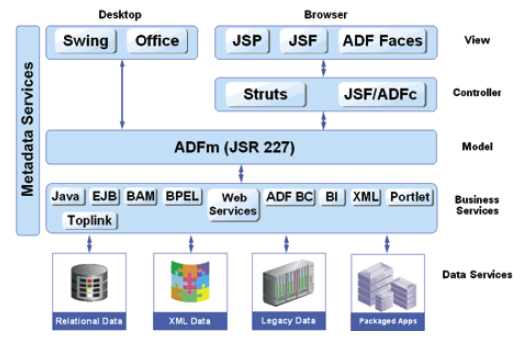
\includegraphics[width=0.80\textwidth]{img/MVC-ADF3.png}
\caption {MVC-Architektur von ADF \autocite[S.22]{AUW2009}}
\label{fig:mvc-adf}
\end{figure}

Die View Ebene der ADF Architektur (siehe Abbildung \ref{fig:mvc-adf}) ist, wie allgemein von der MVC Architektur vorgesehen, die Anzeigeebene der Anwendung und unterteilt sich in die Kategorien Desktop und Browser, da mit ADF sowohl Java Swing Anwendungen (also Desktopanwendungen) als auch Web- oder auch Browser-Anwendungen erstellt werden können \autocite[S.22]{AUW2009}. Diese Unterteilung wirkt sich auch auf die nächste Ebene der Architektur aus, denn eine Trennung von View und Controller wird für Desktopanwendungen nicht zwingend benötigt (siehe auch Kapitel \ref{sec:mvc}). Für Webanwendungen ist es jedoch sinnvoll einen Controller zu haben, um Frontend und Controller getrennt zu behandeln. Der Controller von ADF Anwendungen hat die Aufgabe, Benutzeraktionen zu interpretieren und zu entscheiden, welche Seiten dem User in welcher Reihenfolge angezeigt werden\autocite[S.12]{OAEAD2014}.\\
Das Model ist hier die Abstraktionsschicht. Es besteht aus dem ADF Binding Layer und den Data Controls. Die Data Controls bilden die Schnittstelle zu den Business Services und können daher verschiedene Geschäftslogikimplementierungen zur Verfügung stellen. Der Binding Layer verwendet wiederum die jeweilige vom Data Control zur Verfügung gestellte Geschäftslogik, um mit dem Controller (wenn er vorhanden ist) interagieren zu können und entsprechende Daten im View anzeigen zu können. \autocite[S.6]{ARIA2015}\\
Die beiden zusätzlichen Ebenen in der ADF-MVC-Architektur sind die Business Services und die Data Services. Mit Hilfe dieser Ebenen können in der Anwendung z.B. Web Services angebunden werden und  Verbindungen zu relationalen Datenbanken oder anderen Data Services hergestellt werden \autocite[S.13]{OAEAD2014}. Dies zeigt recht eindeutig, dass es sich bei ADF um ein sehr umfangreiches, nicht modulares Framework handelt, da der Stack der möglichen verwendbaren Technologien von vornherein feststeht und sich auch nicht mehr durch Erweiterungen oder ähnliches verändern lässt.

\subsection{Grails}
\label{sec:grails}
\subsubsection{Grundlegendes}
Auch Grails ist ein Framework, mit dem Web-Anwendungen erstellt werden können. Grails wurde 2005 unter anderem im Zuge der Beliebtheit von auf dynamischen Sprachen basierenden Frameworks entwickelt, die von Ruby on Rails angeführt wurde. Grails basiert auf der 2003 entstandenen Programmiersprache Groovy, die wiederum auf Java basiert\autocite[S.XXV]{DGG2002}\autocite[S.3]{GGR2009}. Das wesentliche Ziel des Frameworks Grails wurde wie folgt beschrieben: \begin{quote}\small "`The goal of Grails is to create a platform with the essence of frameworks like Rails or Django or CakePHP, but one that embraces the mature environment of Java Enterprise Edition(Java EE) and its associated APIs."'\autocite[S.4]{DGG2002}\end{quote} Grails soll also die guten Eigenschaften der bereits bestehenden Frameworks und Java EE verbinden um eine neues mächtiges Framework zu schaffen.

\subsubsection{Architektur}
Auch Grails verwendet, wie ADF und einige weitere Web Frameworks, die MVC-Architektur \autocite[S.208]{GGR2009}. Allerdings hält sich Grails strenger an die im ersten Kapitel beschriebene MVC-Architektur. Es gibt Model, View und Controller die miteinander agieren, wobei der Controller im Fall von Grails nicht optional ist, sondern immer benötigt wird, um eine Interaktion zwischen Model und View zu ermöglichen\autocite[S.8]{DGG2002}.\\
\begin{figure}[H]
\centering
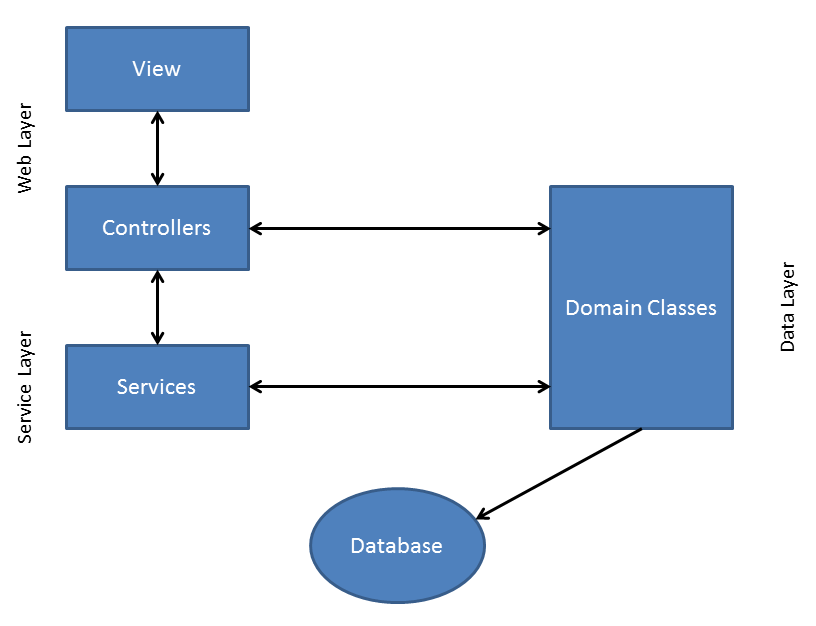
\includegraphics[width=0.80\textwidth]{img/Folie1.png}
\caption {MVC-Architektur von Grails \autocite[S.220]{GGR2009}}
\label{fig:mvc-grails}
\end{figure}
In Abbildung \ref{fig:mvc-grails} sowie auch im Framework selbst wird das Model durch Domain Klassen dargestellt. Diese Klassen sind persistent und werden von Grails automatisch einer jeweils zugehörigen physischen Tabelle in einer Datenbank zugeordnet \autocite[S.17]{DGG2002}. Diese Zuordnung kann zum Beispiel von der im Framework integrierbaren Technologie Hibernate übernommen werden \autocite[S.18]{DGG2002}. Grails lässt jedoch auch andere ORM (Object Relational Mapping) Systeme zu \autocite{GPO2015}. Des weiteren gibt es in Grails, wie auch in ADF die Möglichkeit, Services wie zum Beispiel RESTful Web Services anzubinden. Über die Abbildung (Abbildung \ref{fig:mvc-grails}) hinaus können zudem viele Funktionalitäten zusätzlich über Plugins hinzugefügt und verwendet werden \autocite[S.3]{DGG2002}.\\

In der folgenden Abbildung (Abbildung \ref{fig:tech-stack-grails}) wird der von Grails standardmäßig verwendete Technologiestack dargestellt. Es ist ersichtlich, dass Grails auf der Java Virtual Machine (JVM) aufbaut und Grails durch die verwendete Programmiersprache Groovy zudem die bekannte Java API und die entsprechenden zugehörigen Javadocs mit einem dynamischen Typsystem verbindet. Durch diese Verbindung ist sogar ein Mischen von statischen und dynamischen Typen möglich. \autocite[S.2-4]{DGG2002} 
\begin{figure}[h]
\centering
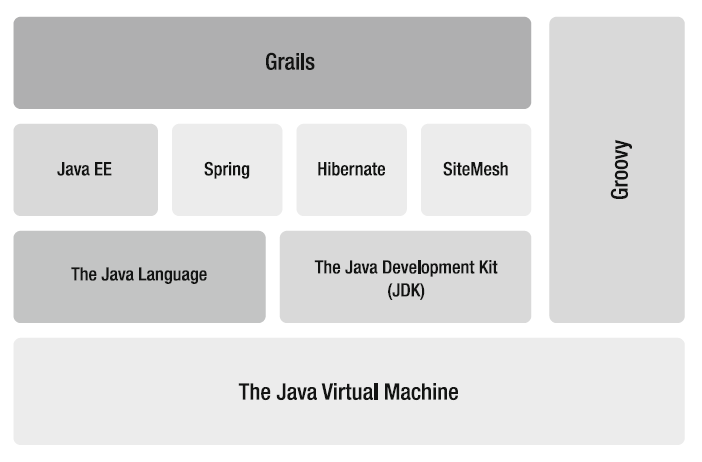
\includegraphics[width=0.80\textwidth]{img/Grails-Stack.png}
\caption {Technologiestack von Grails \autocite[S.3]{DGG2002}}
\label{fig:tech-stack-grails}
\end{figure} 
In Abbildung \ref{fig:tech-stack-grails} ist dies daran zu erkennen, dass sowohl Java als Sprache, als auch das Java Development Kit (JDK) Teil des Grails Technologiestacks sind. Allerdings sind die Komponenten Hibernate und Sitemesh und sogar die Programmiersprache Groovy optional, da statt Groovy auch Java verwendet werden kann und auch für Hibernate oder Sitemesh andere Komponenten verwendet werden können. Damit ist Grails ein sehr modulares Framework \autocite{GP2015}. Standardmäßig beinhaltet der Grails Technologiestack \autocite[S.2]{DGG2002}:
\begin{itemize}
\item Hibernate: Als Standard für objektrelationales Mapping (ORM)
\item Spring: das große und beliebte Open Source Inversion of Control Kontainer und Wrapper Framework für Java
\item SiteMesh: ein robustes und stabiles Layout Rendering Framework
\item Jetty: ein embeddable Servlet Container
\item HSQLDB: Ein reines Java relationales Datenbank Management System (RDBMS) 
\end{itemize}